\documentclass[11pt]{article}

\usepackage[a3paper,margin=0.8in]{geometry}

\usepackage[dvipsnames]{xcolor}
\usepackage{fontspec}
\usepackage{multicol}
\usepackage{amsmath}
\usepackage{tcolorbox}
\usepackage{minted}
\usepackage{mdframed}     % assist minted

%%
% titlesec
%%

\usepackage{titlesec}
\titleformat{\paragraph}[hang]{%
  \normalfont\normalsize\bfseries%
  }{\theparagraph}{1em}{}
\titleformat{\subparagraph}[hang]{%
  \normalfont\small\bfseries%
  }{\thesubparagraph}{1em}{}
  \titlespacing*{\subparagraph}{0pt}{*1}{0pt}

%%
% hyperref
%%

\usepackage[
  colorlinks=true,
  linkcolor=red,
  filecolor=red,
  urlcolor=red,
]{hyperref}

%%
% minted
%%

\usepackage{minted}
\usemintedstyle{colorful}
\BeforeBeginEnvironment{minted}{\begin{mdframed}[
  backgroundcolor=gray!10,
  linecolor=gray!40,
]}
\AfterEndEnvironment{minted}{\end{mdframed}}
\setminted{
  frame=lines,
  framesep=2mm,
  baselinestretch=1.2,
  linenos,
  breaklines=true,
  fontsize=\footnotesize,
}

%%
% Document-specific commands (mostly abbreviations)
%%

\newcommand{\lbtlabel}{\textsf{lbt}} 
\newcommand{\lbtpkg}{\texttt{lbt}} 

%%%%%%%%%%%%%%%%%%%%%%%%%%%%%%%%%%%%%%%%%%%%%%%%%%%%%%%%%%%%%%%%%%%%%%%%
%
%%%%%%%%%%%%%%%%%%%%%%%%%%%%%%%%%%%%%%%%%%%%%%%%%%%%%%%%%%%%%%%%%%%%%%%%

\begin{document}

\title{The \textbf{lbt} (Lua-based templates) package}
\author{%
  Gavin Sinclair\\%
  gsinclair@gmail.com\\%
  github.com/gsinclair/lbt%
}
\date{v0.1~from 2023/12/03}

\maketitle

\vfill

\setcounter{secnumdepth}{5}
\setcounter{tocdepth}{5}
\tableofcontents

\vfill
\clearpage

%-----------------------------------------------------------------------
% Introduction
%-----------------------------------------------------------------------

\pagebreak

% --------------------------------------------------------------------------------
% # Introduction -----------------------------------------------------------------
% --------------------------------------------------------------------------------

\section{Introduction}

\LaTeX{} is a formidible document processing software package. The input language is generally suited to its task and is flexible, but it does have some shortcomings.
\begin{itemize}
  \item Major structural concepts are coded the same way as minor formatting concepts, for instance \verb|\section{Pre-war Japan}| and \verb|\emph{The Seven Samurai}|. Thus it can be difficult to read a Latex file and see the structure.
  \item When it comes to structured content, even simple items like an exam question require a lot of boilerplate.
\end{itemize}

\textcolor{blue}{\lbtpkg{} is a Lua\LaTeX{} package that allows authors to write structured content (e.g.~course handouts, exams, worksheets) more easily by using templates.} The templates control overall appearance of a section of a document (e.g.~new page, title, colour, etc.) and also provide for easy writing of the elements of the document.

Importantly, a template comprises only \emph{part} of a \LaTeX{} document, so you can still set out your overall document---chapters, sections, general text---in a normal way.

An example will help to convey the purpose and the power. Figure~\ref{fig:example1code} shows some idiomatic \LaTeX{} code to write a couple of exam questions, and the equivalent code written using \lbtlabel{}. Figure~\ref{fig:example1out} shows the result.\footnote{To be clear, the two pieces of code are not exactly equivalent, as the \lbtlabel{} code does not use the \texttt{exam} package in the background.}


\begin{figure}
\begin{tcolorbox}
\small\color{blue!55}
\begin{verbatim}
\begin{questions}
\question Einstein's famous formula is $E = mc^2$.
\begin{parts}
\part Calculate the energy equivalent of 2.8\,g of mass.
\part Which of the following is NOT a correct rearrangement of the formula?
\begin{choices}
\choice $m = E/c^2$
\choice $c = \sqrt{E/m}$
\choice $c = Em^2$ :: $c^2 = M/e$
\choice $c^2 = M/e$
\end{choices}
\end{parts}
\end{questions}
\end{verbatim}
\tcblower
\small\color{blue!80}
\begin{verbatim}
Q Einstein's famous formula is $E = mc^2$.
QQ Calculate the energy equivalent of 2.8\,g of mass.
QQ Which of the following is NOT a correct rearrangement of the formula?
MC $m = E/c^2$ :: $c = \sqrt{E/m}$ :: $c = Em^2$ :: $c^2 = M/e$
\end{verbatim}
\end{tcolorbox}
\caption{Questions for a worksheet or exam written in ordinary \LaTeX{} using \textsf{exam}, followed by equivalent content written using \lbtlabel{}.}
\label{fig:example1code}
\end{figure}

\begin{figure}
\begin{tcolorbox}
  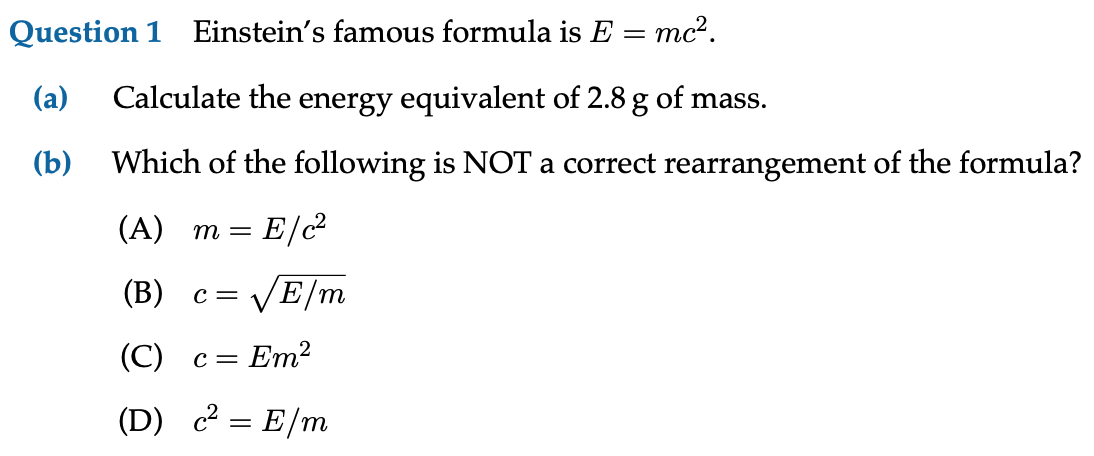
\includegraphics[width=0.8\textwidth]{media/example1.png}
\end{tcolorbox}
\caption{Sample output.}
\label{fig:example1out}
\end{figure}



% --------------------------------------------------------------------------------
% # Understanding the design and implementation ----------------------------------
% --------------------------------------------------------------------------------

\section{Understanding the design and implementation}

We take a horizontal and vertical look at the ideas and implementation. These two views can be considered in either order.
\begin{itemize}
  \item A horizontal look examines the code one file at a time, and so all concerns are intermingled.
  \item A vertical look takes one concept at a time and describes the implementation top-down.
\end{itemize}

% --------------------------------------------------------------------------------
% ## A horizontal look -----------------------------------------------------------

\subsection{A horizontal look}

The code in this section does \emph{not} represent the actual package code. It is a curated presentation of the package code early in its development. From this code we can learn the fundamentals of the code structure.

% ## lbt.sty ---------------------------------------------------------------------

\subsubsection{\texttt{lbt.sty}}

Lines 1--7 set out the name of the class, some version information, and some packages that are required for it to operate.

Lines 9--11 consider options that may be passed. Processing options is an important part of writing a package, but this is deferred until later. It would be nice to be able to write \mintinline{latex}|\usepackage[draft]{lbt}|.

Lines 13--30 are a chunk of Lua code that really sets things up. We load the \textsf{penlight} Lua library, which provides a lot of generally useful functions, and we set up the global \lbtpkg{} table, which contains data and functions.
\begin{itemize}
  \item Line 15 alters the Lua package path so that we can load \textsf{penlight} from the \texttt{vendor} directory. Line 16 loads \textsf{penlight} in such a way that its many modules will now be auto-loaded on demand by simply using (for example) \texttt{pl.util.split} or \texttt{pl.file.move}.
  \item Lines 17--18 monkey-patch the Lua \texttt{string} and \texttt{table} modules with all the extra \textsf{penlight} goodness.
  \item Line 21 prints a message to the Latex output/log just so we can see this code is running.
  \item Line 22 creates the global table \lbtpkg{}. All \lbtlabel{} functionality lives in here, so that we minimise our effect on the global environment.
  \item Lines 23--28 load the Lua files that implement the package functionality. They are split for ease of development and maintenance. In general, each file sets up a different part of the \lbtpkg{} table.
  \item Line 29 writes a message to the log file \texttt{lbt.log} using the function \texttt{lbt.log(...)} that was created in \texttt{lbt-0-meta.lua}. This helps us to see that things have been set up at least somewhat correctly.
\end{itemize}

Lines 32--38 indicate Latex commands and environments that will likely be implemented in future. We can see here the use of \texttt{lbt.api}, which is the collection of Lua functions that should be called from Latex. The \lbtpkg{} environment calls \texttt{clear\_content()} to provide a blank slate for processing to begin, and \texttt{emit\_tex()} to process the written content contained in the \lbtpkg{} environment and output the required Latex code into the stream. The \texttt{lbtResetChapterCounters} Latex command also calls a Lua function in \texttt{lbt.api}.

\inputminted{latex}{media/impl-lbt.sty}

The \textbf{key takeaways from this code} are:
\begin{itemize}
  \item All Lua data and functionality is contained within the global table \lbtpkg{}.
  \item The \lbtlabel{} package loads its own copy of the \textsf{penlight} library and uses the global variable name \texttt{pl} to access its features.
  \item The \texttt{string} and \texttt{table} modules have extra functions added to them.
\end{itemize}

If you use your own Lua code in conjuntion with \lbtlabel{} then you will want to be aware of these impacts on the global environment. If the monkey-patching of \texttt{string} and \texttt{table} are inconvenient for you, let me know and perhaps a future version can tread more lightly.

% ## lbt-0-meta.lua---------------------------------------------------------------

\subsubsection{\texttt{lbt-0-meta.lua}}

In this first Lua file to be loaded, we set some information \emph{about} the Lua module, and we create functions for logging and debugging to the files \texttt{lbt.log} and \texttt{lbt.dbg} respectively.

The code and comment in lines 1--13 was borrowed from the \textsf{cloze} package by Josef Friedrich. It is probably not being used correctly, but is here for now so I don't forget to research it properly later.

\inputminted{lua}{media/impl-lbt-0-meta.lua}

The \textbf{key takeaways from this code} are:
\begin{itemize}
  \item The \lbtlabel{} table has two functions defined: \texttt{log} and \texttt{dbg}.
  \item This is unusual. As we shall see, functions are normally defined in sub-tables like \texttt{lbt.util} or \texttt{lbt.api}. But logging and debugging need to be easy to access, and they don't fit naturally elsewhere.
\end{itemize}

% ## lbt-1-init.lua---------------------------------------------------------------

\subsubsection{\texttt{lbt-1-init.lua}}

Here we properly \emph{initialise} the \lbtpkg{} table. The comments are descriptive enough, but for a quick overview, we have a table \texttt{lbt.state} that keeps all necessary variables (current content being processed, counters, modes, \dots) and several tables \texttt{lbt.\{api,fn,util,test\}} that will contain functions.

\inputminted{lua}{media/impl-lbt-1-init.lua}

The \textbf{key takeaways from this code} are:
\begin{itemize}
  \item Data is separated into three groups: \texttt{system} data that persists for the life of the Latex document; \texttt{const} and \texttt{var} data pertinent to the current expansion.
  \item Functions are separated into groups by purpose.
  \item \texttt{api} functions are to be called by Latex code.
  \item \texttt{fn} functions support the API directly.
  \item \texttt{util} functions support the implementation and/or templates.
  \item \texttt{test} functions provide for some testing.
  \item \texttt{init} functions initialise the state (\texttt{const} and \texttt{var}) for a new expansion.
\end{itemize}

Note that we \emph{specify} these function groups in a top-down manner, but will implement them bottom-up.

% ## lbt-2-util.lua---------------------------------------------------------------

\subsubsection{\texttt{lbt-2-util.lua}}

The \texttt{util} functions will be useful support for the implementation of the \lbtlabel{} module and also to document authors who need to implement templates. The two functions shown below are just a start.

Note the use of \textsf{penlight} functions in lines 12 and 13. Basic Lua does not have ergonomic support for checking types or getting lines from a string.

\inputminted{lua}{media/impl-lbt-2-util.lua}

% ## lbt-3-fn.lua ----------------------------------------------------------------

\subsubsection{\texttt{lbt-3-fn.lua}}

The \texttt{fn} functions support the implementation of the \lbtlabel{} module directly. The single function shown below, included for demonstration purposes, is from an earlier version of the code. It finds all template (Lua) files in a \texttt{templates} directory, loads each one, and builds a table such as \mintinline{lua}|{ "Worksheet" = <template code>, "CourseHandout" = <template code>, "FundingRequest" = <template code>, ...}|.

The function is out of date because the template directory is mixed in with the project files, which is no longer possible because templates will need to reside on a user's machine. However, it is included here to give a flavour of \texttt{fn} functions. Some things to point out are:
\begin{itemize}
  \item the use of \textsf{penlight} on line 6;
  \item the use of \texttt{lbt.state} on lines 11, 18, 24, 25;
  \item debugging with \texttt{lbt.dbg} on lines 19, 21, 22.
\end{itemize}

\inputminted{lua}{media/impl-lbt-3-fn.lua}

% ## lbt-4-api.lua ---------------------------------------------------------------

\subsubsection{\texttt{lbt-4-api.lua}}

The functions in \texttt{api} are to be called by Latex code in \texttt{lbt.sty}. They are brief because they are often simple (get/set some state). When they are not simple, they just check argument types and defer to code in \texttt{fn}. This means we can see all of the API at a glance. The code shown here is not complete.

The absolute heart of the whole package is shown in lines 8--31.

\inputminted{lua}{media/impl-lbt-4-api.lua}

The \textbf{key takeaways from this code} are:
\begin{itemize}
  \item The three key functions that support \mintinline{latex}|\begin{lbt} ... \end{lbt}| are:
  \begin{itemize}
    \item \texttt{clear\_content};
    \item \texttt{process};
    \item \texttt{emit\_tex}.
  \end{itemize}
  \item Other functionality on display here includes draft/debug mode, counters, and ``data'' (a generalisation of counters).
\end{itemize}

% ## lbt-5-err.lua ---------------------------------------------------------------

\subsubsection{\texttt{lbt-5-err.lua}}

In order to give good error messages when a user makes mistakes implementing or using a template, all error handling is centralised in this module.

\textbf{NOTE:} the implementation shown below is incredibly juvenile and will be refined both in the real code and in this documentation as time goes on.

\inputminted{lua}{media/impl-lbt-5-err.lua}

The \textbf{key takeaways from this code} are:
\begin{itemize}
  \item xxx
  \item xxx
\end{itemize}

% ## lbt-6-builtin-templates.lua -------------------------------------------------

\subsubsection{\texttt{lbt-6-builtin-templates.lua}}

There are some templates that are built into \lbtlabel{}. We show the code for the most fundamental of them here.

The \texttt{Basic} template implements a suite of \LaTeX{} functionality. It implements commands but not layout. The commands in this template are always available; you never need to import \texttt{Basic}. As an example, using this template you could write the following in your document. The content would appear inline, surrounded by whatever other Latex you have written.

\begin{minted}{text}
  @META
      TEMPLATE    Basic

  + BODY
      TEXT When I go shopping \textbf{this afternoon}, I will buy:
      ITEMIZE topsep=0mm ::
      » \item dog food;
      » \item large pedestal fan;
      » \item chlorine for the swimming pool.
      VSPACE 30pt
      COMMENT I also want a pistachio croissant, but the patisserie is closed.

      CLEARPAGE

      NEWCOMMAND signature :: 2 :: \hfill \textcolor{blue}{---#1 (\emph{#2})}
      BEGIN multicols 2
      TEXT To be, or not to be, that is the question: \\
      » Whether 'tis nobler in the mind to suffer \\
      » The slings and arrows of outrageous fortune, \\
      » Or to take arms against a sea of troubles \\
      » And by opposing end them. To die—to sleep, \\
      » No more; and by a sleep to say we end \\
      » The heart-ache and the thousand natural shocks \\
      » That flesh is heir to: 'tis a consummation \\
      » Devoutly to be wish'd. To die, to sleep; \\
      » To sleep, perchance to dream—ay, there's the rub: \\
      » For in that sleep of death what dreams may come, \\
      » When we have shuffled off this mortal coil, \\
      » \dots
      » \signature{Shakespeare}{Hamlet}
      END multicols
\end{minted}

The following features demonstrated, in order.
\begin{itemize}
  \item Ordinary text, which forms a paragraph and can include ordinary Latex commands like \verb|\textbf{...}|.
  \item An itemised list, complete with optional arguments to the \texttt{enumitem} package.
  \item Vertical space.
  \item A comment, which will be ignored.
  \item Clearing the page to start a new one. Note that if \texttt{CLEARPAGE} were not defined then the result could still be achieved like so: \texttt{CMD clearpage}.
  \item A new command is defined on line 15 and used on line 30.
  \item An environment -- in this case, \texttt{multicols} -- with \texttt{BEGIN} and \texttt{END}.
  \item The use of the » character to signal line continuation.
\end{itemize}

The code below shows how these features are implemented (except the line continuation, which is lower-level syntax): they are Lua functions that take input text and return a string of Latex code. In the case of \texttt{BEGIN} and \texttt{NEWCOMMAND} (and two others), the function body splits the text on \texttt{::} and handles the arguments. This is an example of using a programming language (Lua) to do macro logic instead of the (La)TeX language.

At the bottom of the file, the actual template is created using \texttt{lua.api.make\_template}. The \texttt{Basic} template has no need for initialisation or expanding, so this declaration is very simple.

\inputminted{lua}{media/impl-lbt-6-builtin-templates.lua}

The \textbf{key takeaways from this code} are:
\begin{itemize}
  \item Commands in the \lbtlabel{} template language map directly to Lua functions in a table. If you need a template for writing a textbook, you might design commands like \texttt{EXAMPLE} and \texttt{EXERCISE}, and these would simply be implemented by Lua functions of the same name.
  \item The Lua functions receive a single string, which might be empty (e.g. \texttt{CLEARPAGE}), or have a simple argument (e.g. \texttt{VSPACE 30pt} or \texttt{TEXT When I go shopping...}), or have multiple arguments that need to be separated (e.g. \texttt{BEGIN multicols 2} or \texttt{ITEMIZE topsep=0mm :: ...}).
  \item There is builtin support for separating the arguments and checking there is an appropriate number of them: \texttt{lbt.util.arguments()}.
  \item The bulk of writing a template might be defining functions, but the tempate itself needs to be registered in the system, hence \texttt{lbt.api.make\_template}.
\end{itemize}

Another important fact to emphasise here is that most templates involve holistic formatting. A business letter has several details: to, from, address, date, salutation, letterhead graphic. An educational worksheet could have a title, course, optional date, teacher's notes (on a separate page), questions, answers. See \textcolor{red}{todo!} for examples of these.

% ## lbt-7-test.lua ---------------------------------------------------------------

\subsubsection{\texttt{lbt-7-test.lua}}

\textbf{NOTE:} This section is yet to be written.

% --------------------------------------------------------------------------------
% ## A vertical look -------------------------------------------------------------

\subsection{A vertical look}

Another way of looking at the design and implementation is to take one concept at a time and discuss its implementation from top to bottom.

% ### Specifying the template ----------------------------------------------------

\subsubsection{Specifying the template}

% ### Which templates are included? ----------------------------------------------

\subsubsection{Which templates are included?}

% ### Draft mode and debug mode --------------------------------------------------

\subsubsection{Draft mode and debug mode}

% ### Processing the author's input ----------------------------------------------

\subsubsection{Processing the author's input}

% ### Emitting the Latex ---------------------------------------------------------

\subsubsection{Emitting the Latex}

\pagebreak

% --------------------------------------------------------------------------------
% # Introduction -----------------------------------------------------------------
% --------------------------------------------------------------------------------

\section{Old implementation}

\subsection{gsContent.lua}

\inputminted{lua}{media/gsContent.lua}

\subsection{gsHelpers.lua}

\inputminted{lua}{media/gsHelpers.lua}

\subsection{gsLatex.tex}

\inputminted{latex}{media/gsLatex.tex}

\subsection{gsMisc.lua}

\inputminted{lua}{media/gsMisc.lua}

\subsection{gsMisc.tex}

\inputminted{latex}{media/gsMisc.tex}

\end{document}
